\documentclass[output=paper,colorlinks,citecolor=brown,modfonts,nonflat]{langsci/langscibook}
\ChapterDOI{10.5281/zenodo.3776547}
\author{Egor Tsedryk\affiliation{Saint Mary’s University}}
\title{The modal side of the dative: From predicative possession to possessive modality}
\abstract{This chapter examines predicative possession (e.g., I have a book) in relation to possessive modality (e.g., I have to buy a book) (\citealt{Bhatt1997, BjorkmanCowper2016}). \citet{BjorkmanCowper2016} report that in Hindi-Urdu and Bengali (\textsc{be}-languages), possessive modality consistently correlates with the dative case, whereas predicative possession allows other obliques, namely genitive. They propose that both predicative possession and possessive modality are reducible to an interpretable feature encoding inclusion, [\textsc{incl}], and suggest that the dative case is a morphosyntactic realization of [\textsc{incl}] combined with a modal operator within a single syntactic head via featural composition. Focusing on Russian – another \textsc{be}{}-language – I show that there are problems with this analysis. Russian data indicates that possessive modality in this language is to be derived from directional (vector-like) semantics of the head that introduces the dative. I offer a unified account of the dative used with an NP and the one used with a TP, assuming a single argument-introducing head, \textit{i}* (\citealt{WoodMarantz2017}).
% \textbf{Keywords:} \textit{possession, modality, inclusion, directional meaning, dative infinitive construction, Russian}
}

\IfFileExists{../localcommands.tex}{
  % add all extra packages you need to load to this file  
\usepackage{tabularx} 
\usepackage{url} 
\urlstyle{same}

\usepackage{listings}
\lstset{basicstyle=\ttfamily,tabsize=2,breaklines=true}


%%%%%%%%%%%%%%%%%%%%%%%%%%%%%%%%%%%%%%%%%%%%%%%%%%%%
%%%                                              %%%
%%%           Examples                           %%%
%%%                                              %%%
%%%%%%%%%%%%%%%%%%%%%%%%%%%%%%%%%%%%%%%%%%%%%%%%%%%% 
%% to add additional information to the right of examples, uncomment the following line
% \usepackage{jambox}
%% if you want the source line of examples to be in italics, uncomment the following line
% \renewcommand{\exfont}{\itshape}
\usepackage{langsci-optional}
\usepackage{./langsci/styles/langsci-gb4e}
\usepackage{./langsci/styles/langsci-lgr}
\usepackage{pgfplots,pgfplotstable}

\definecolor{lsDOIGray}{cmyk}{0,0,0,0.45}

\usepackage{xassoccnt}
\newcounter{realpage}
\DeclareAssociatedCounters{page}{realpage}
\AtBeginDocument{%
  \stepcounter{realpage}
}


 



 

  \newcommand{\appref}[1]{Appendix \ref{#1}}
\newcommand{\fnref}[1]{Footnote \ref{#1}} 

\newenvironment{langscibars}{\begin{axis}[ybar,xtick=data, xticklabels from table={\mydata}{pos}, 
        width  = \textwidth,
	height = .3\textheight,
    	nodes near coords, 
	xtick=data,
	x tick label style={},  
	ymin=0,
	cycle list name=langscicolors
        ]}{\end{axis}}
        
\newcommand{\langscibar}[1]{\addplot+ table [x=i, y=#1] {\mydata};\addlegendentry{#1};}

\newcommand{\langscidata}[1]{\pgfplotstableread{#1}\mydata;}

\makeatletter
\let\thetitle\@title
\let\theauthor\@author 
\makeatother

\newcommand{\togglepaper}[1][0]{ 
%   \bibliography{../localbibliography}
  \papernote{\scriptsize\normalfont
    \theauthor.
    \thetitle. 
    To appear in: 
    Change Volume Editor \& in localcommands.tex 
    Change volume title in localcommands.tex
    Berlin: Language Science Press. [preliminary page numbering]
  }
  \pagenumbering{roman}
  \setcounter{chapter}{#1}
  \addtocounter{chapter}{-1}
}
\newcommand{\orcid}[1]{}

  %% hyphenation points for line breaks
%% Normally, automatic hyphenation in LaTeX is very good
%% If a word is mis-hyphenated, add it to this file
%%
%% add information to TeX file before \begin{document} with:
%% %% hyphenation points for line breaks
%% Normally, automatic hyphenation in LaTeX is very good
%% If a word is mis-hyphenated, add it to this file
%%
%% add information to TeX file before \begin{document} with:
%% %% hyphenation points for line breaks
%% Normally, automatic hyphenation in LaTeX is very good
%% If a word is mis-hyphenated, add it to this file
%%
%% add information to TeX file before \begin{document} with:
%% \include{localhyphenation}
\hyphenation{
affri-ca-te
affri-ca-tes
Tarra-go-na
Vio-le-ta
Jacken-doff
clit-ics
Giar-di-ni
Mor-fo-sin-tas-si
mi-ni-mis-ta
nor-ma-li-tza-ció
Caus-ees
an-a-phor-ic
caus-a-tive
caus-a-tives
Mar-antz
ac-cu-sa-tive
Ma-no-les-sou
phe-nom-e-non
Holm-berg
}

\hyphenation{
affri-ca-te
affri-ca-tes
Tarra-go-na
Vio-le-ta
Jacken-doff
clit-ics
Giar-di-ni
Mor-fo-sin-tas-si
mi-ni-mis-ta
nor-ma-li-tza-ció
Caus-ees
an-a-phor-ic
caus-a-tive
caus-a-tives
Mar-antz
ac-cu-sa-tive
Ma-no-les-sou
phe-nom-e-non
Holm-berg
}

\hyphenation{
affri-ca-te
affri-ca-tes
Tarra-go-na
Vio-le-ta
Jacken-doff
clit-ics
Giar-di-ni
Mor-fo-sin-tas-si
mi-ni-mis-ta
nor-ma-li-tza-ció
Caus-ees
an-a-phor-ic
caus-a-tive
caus-a-tives
Mar-antz
ac-cu-sa-tive
Ma-no-les-sou
phe-nom-e-non
Holm-berg
}

  \bibliography{../localbibliography}
  \togglepaper[8]%%chapternumber
}{}

\begin{document}
\maketitle
\shorttitlerunninghead{The modal side of the dative}

\section{Background}\label{sec:tsedryk:1}

The \textsc{be} + \textsc{oblique} pattern in \textsc{be}-possession languages, or \textsc{be}{}-languages \citep{Isačenko1974} has been taken as evidence to support a unified analysis of possession and necessity, as in \REF{ex:tsedryk:1}, an example from Bengali \citep[43]{BjorkmanCowper2016}. \citet[31]{BjorkmanCowper2016} use the term “possessive modality” to refer to constructions like \REF{ex:tsedryk:1b}, which express modal necessity and have a morphosyntactic resemblance to predicative possession.

\ea%1
    \label{ex:tsedryk:1}
    \ea\label{ex:tsedryk:1a}
    \gll    \textbf{Amar}    \textbf{bondhu-r}     {akʈa}   {boi}     {aatʃhe}.\\
            my       friend-\textsc{gen}  one     book   be.\textsc{prs}\\
    \glt    ‘My friend has a book.’
    \ex\label{ex:tsedryk:1b}
    \gll    \textbf{Amar}    \textbf{bondhu-ke}    {je-te}     {ho-be}.\\
            my friend-\textsc{dat}    go-\textsc{inf}   be-\textsc{fut}\\
    \glt    ‘My friend has to leave.’
    \z
\z


Note that there is a discrepancy in the case marking of the bolded DPs in \REF{ex:tsedryk:1a} and \REF{ex:tsedryk:1b}. Interestingly, possessive modality consistently correlates with the dative case.\footnote{\citet[example 7]{Bhatt1997} reports a case of possessive modality in Bengali with a genitive subject. However, \citet[46]{BjorkmanCowper2016} report that the dative case is the preferred option in their informant’s dialect.} As \citet[section 8.1]{Bhatt1997} suggests, the dative could be related to a lack of control over a situation, but he does not develop this idea any further.\footnote{The same idea is also recurrent in the literature dealing with so-called “involuntary state constructions” in Slavic (\citealt[154]{Rivero2009}; \citealt[312]{RiveroArregui2012}).}

\citet{Bhatt1997} offers an account of possessive modality, relying on the idea that \textsc{have} is a result of incorporating a “prepositional determiner” (D/P) into the underlying verb \textsc{be} (following \citealt{Freeze1992} and \citealt{Kayne1993}). Along the lines of \citeauthor{Kayne1993}’s analysis, a sentence like \textit{I have a book} has the structure in \REF{ex:tsedryk:2a} (several technical details being put aside). The possessor (Subj) is base-generated with the possessee (within an agreement phrase), and it has to move for case reasons. In \textsc{be}{}-languages, the specifier position of D/P is a case position, but in \textsc{have-}languages, it is not. Thus, Subj is forced to move further. Spec,DP is assumed to be an A'{}-position and, in order to avoid improper movement, D/P has to incorporate into \textsc{be} (I am not going to expand on this idiosyncrasy of \citeauthor{Kayne1993}’s analysis; see \citealt[320–328]{Myler2016} for an overview and a critical assessment). A sentence like \textit{I have to buy a book}, on the other hand, has the structure in \REF{ex:tsedryk:2b}, which is very similar to \REF{ex:tsedryk:2a}. The only difference is in the type of D/P’s complement: in \REF{ex:tsedryk:2b}, it is a proposition with a modal operator (Mod).

\ea%2
    \label{ex:tsedryk:2}
    \ea\label{ex:tsedryk:2a}{}
    [Subj\textsubscript{i} \textsc{be} [\textsubscript{DP} t'\textsubscript{i} D/P [\textsubscript{AgrP} t\textsubscript{i} \textit{a book}]]]
    \ex\label{ex:tsedryk:2b}{}
    [Subj\textsubscript{i} \textsc{be} [\textsubscript{DP} t'\textsubscript{i} D/P [\textsubscript{ModP} Mod [\textit{to} [t\textsubscript{i} \textit{buy a book}]]]]]
    \z
\z

According to this analysis, possessive modality expresses a relation between an individual and a proposition containing a modal operator: \textit{I have (an obligation) to buy a book}.

\citet{BjorkmanCowper2016} on the other hand, argue against a modal operator in the propositional component of possessive modality. They analyze possession and necessity in terms of inclusion. The latter is not formally defined, but the basic idea is expressed in the following lines:

\begin{quote}
Though \textit{inclusion} or \textit{part-whole} seems to be a reasonable relation to postulate in the domain of inalienable possession, [... a] potentially more interesting possibility is that abstract possession relations, such as alienable possession and kinship relations, can also be usefully seen as involving some kind of inclusion or containment. [...] A clear statement of this type of intuition can be found, for example, in the following lines from \citet{BonehSichel2010}:

\begin{quote}
“We take Part-Whole to be broader than inalienable possession and to include also social relations and inanimate Part-Whole” (pp. 2–3)

“[T]he complement of the applicative head [= a subset of possessees] can be understood as \textbf{falling} \textbf{within} \textbf{the} \textbf{sphere} of the applied argument.” (p. 28, emphasis ours)
\end{quote}

The idea of containment within a sphere of influence, expressed in the second of these quotes, suggests a possible link between inclusion and the notion of \textit{control}, discussed in the context of typological work on possession by authors such as \citet{Heine1997} and \citet{Stassen2009}. \citep[33--34]{BjorkmanCowper2016}
\end{quote}

\citeauthor{BjorkmanCowper2016} propose to formalize inclusion as a morphosemantic feature, [\textsc{incl}], specifying a functional verbal/applicative-like head, labeled as little \textit{v}  (cf. ${\subseteq}$ and ${\supseteq}$ in \citetv{chapters/franco}). According to \citeauthor{BjorkmanCowper2016}, [\textsc{incl}] is responsible for the projection of an asymmetric structure, in which the possessor (“the applied argument” in the passage above) asymmetrically c-commands the complement of the head bearing this feature.

The link between predicative possession and possessive modality (modal necessity) is captured as follows. In the case of predicative possession, [\textsc{incl]} relates individuals, or arguments of type \textit{e} (possessor and possessee). There are two options for {\liv}[\textsc{incl}] in \REF{ex:tsedryk:3}: it can assign case to its complement (in \textsc{have}\textit{{}-}languages) or it can introduce an oblique argument in the specifier of {\liv}[\textsc{incl}] (in \textsc{be}{}-languages).

\ea%3
    \label{ex:tsedryk:3}
\begin{forest}  fairly nice empty nodes
[{\liv}P
    [Possessor]
    [
        [{\liv}\\\textsc{[incl]}]
        [Possessee]
    ]
]
\end{forest}
    \z

In the case of possessive modality, the arguments related by [\textsc{incl]} are sets of worlds, or arguments of type {\textlangle}\textit{s}, \textit{t}{\textrangle}: (i) a set of accessible worlds of the modal base and (ii) a set of worlds in which a given proposition is true (the first set is a subset of the second). According to \citeauthor{BjorkmanCowper2016}, whenever inclusion is extended from individuals to sets of worlds, the syntactic realization of these arguments changes as well. More precisely, the argument associated with accessible worlds is realized as a modal feature on the head that bears [\textsc{incl}]: either [\textsc{root}] or [\textsc{epist}] (epistemic). That is, the semantic co-argument of the proposition is not merged in the specifier position of \textit{v} (\textit{v} is an intransitive head in this case); the latter hosts the subject raising out of the proposition.

\ea%4
    \label{ex:tsedryk:4}
\begin{forest} fairly nice empty nodes
[{\liv}P
    [Subj]
    [
        [{\liv}\\\textsc{[incl]}\\\textsc{[root/epist]}]
        [Proposition [… {\textlangle}Subj{\textrangle} …, roof]]
    ]
]
\end{forest}
    \z

Finally, different combinations of features result in different realizations in morphology. In English – and hypothetically other \textsc{have}{}-languages – {\liv}[\textsc{incl}] is realized as \textit{have} irrespectively of whether or not there is an additional modal feature. In Bengali – and hypothetically other \textsc{be}{}-languages – [\textsc{incl}] is realized in the specifier position, based on the following rules (\citealt{BjorkmanCowper2016}: 46).

\ea%5
    \label{ex:tsedryk:5}
    \ea\label{ex:tsedryk:5a}
    {\liv}\textsc{[incl][root/epist]} → \textsc{dat}
    \ex\label{ex:tsedryk:5b}
    {\liv}\textsc{[incl]} → \textsc{gen}
    \z
\z

In other words, languages are expected to vary with regard to the degree of feature specification in morphology and the locus of the morphosyntactic realization of [\textsc{incl]} and other features it is paired with (specifier or head + complement).

Generally, I agree with \citeauthor{BjorkmanCowper2016}’s analysis of \textsc{have} in both predicative possession and possessive modality, but I disagree with their treatment of the dative case in \textsc{be}{}-languages, at least in a subset of such languages. Their analysis might be a good fit for Hindi/Bengali, but I will show that it faces problems when applied to a \textsc{be}-language like Russian. These problems are discussed in \sectref{sec:tsedryk:2}. As we will see, Russian has predicative possession with both a locative (actual) possessor and a dative (possible/prospective) possessor. The former is indeed the bearer of feature [\textsc{incl}], but the latter has a purely directional meaning (‘towards’). It is the latter that I propose to link to possessive modality, not the former. Following \citet{TsedrykInPress}, I use \citegen{WoodMarantz2017} single argument-introducing head in my analysis of both possessors. \sectref{sec:tsedryk:3} elaborates on such notions as “sphere” and “control”, mentioned in the excerpt from \citet{BjorkmanCowper2016}, preceding \REF{ex:tsedryk:3} above. In \sectref{sec:tsedryk:4}, I use the same argument introducer in my analysis of possessive modality in Russian. Finally, \sectref{sec:tsedryk:5} concludes.

\section{ Focus on Russian}\label{sec:tsedryk:2}

\subsection{Overview}\label{sec:tsedryk:2.1}

In \REF{ex:tsedryk:6}, I provide a Russian equivalent of a pair like the one in \REF{ex:tsedryk:1}, presenting predicative possession in \REF{ex:tsedryk:6a} and possessive modality in \REF{ex:tsedryk:6b}. The latter example illustrates a so-called “dative infinitive” construction expressing modal necessity, which – according to \citeauthor{BjorkmanCowper2016} – is a prerequisite of possessive modality.\footnote{\citeauthor{BjorkmanCowper2016} (footnote 18) briefly mention Russian, but the only example they provide is a \textit{wh}{}-question in (i) (from \citealt[105]{Jung2011}). As shown in \citet{Tsedryk2018} (see also \citealt{Fortuin2007}), Russian dative infinitive constructions may have different modal flavours (necessity, ability and deontic flavours), depending on the morphosyntactic makeup of the clause (see \sectref{sec:tsedryk:4}).

\ea%i
    \gll    Začem  mne       bylo          tam     ostavat’sja?\\
            why     me.\textsc{dat}   be.\textsc{pst.n.sg}  there   stay.\textsc{inf}\\
    \glt    ‘Why was I supposed to stay there?’
\z

Moreover, \citet[ch. 4]{Bhatt2006} has shown that infinitival questions in English exhibit a variable modal behaviour (\textit{could}, \textit{would} or \textit{should}), depending on the context and the embedding verb (e.g., \textit{Ásta knows where to get gas, Ásta decided where to get gas}, \textit{Ásta told Hafdis where to get gas}; see \citealt[124]{Bhatt2006}). In other words, infinitival questions are not a perfect testing ground for modal necessity or possessive modality, as defined by \citeauthor{BjorkmanCowper2016}.}

\ea%6
    \label{ex:tsedryk:6}
    \ea\label{ex:tsedryk:6a}
    \gll    \textbf{U}  \textbf{menja}     {est’}           {kniga}.\\
            at  me.\textsc{gen}   be.\textsc{exist}    book.\textsc{nom}\\
    \glt    ‘I have a book.’
    \ex\label{ex:tsedryk:6b}
    \gll    \textbf{{Mne}}      {zavtra}       {rano}   {vstavat’}.\\
            me.\textsc{dat}  tomorrow  early  get.up.\textsc{ipfv.inf}\\
    \glt    ‘I have to get up early tomorrow.’ \hfill \citep[ex. (20a)]{Tsedryk2018}
    \z
\z

To apply \citeauthor{BjorkmanCowper2016}’s analysis, we would have to assume that the existential light verb ({\liv}\textit{\textsubscript{exist}}) in \REF{ex:tsedryk:6a} bears feature [\textsc{incl}], which is responsible for the merger of the locative PP in Spec,{\liv}P, as shown in \REF{ex:tsedryk:7a}. As for \REF{ex:tsedryk:6b}, it would have the structure in \REF{ex:tsedryk:7b}, where [\textsc{incl}] is clustered with feature [\textsc{root}], responsible for the dative case assigned to the subject raised to Spec,{\liv}P.

\ea%7
    \label{ex:tsedryk:7}
    \ea\label{ex:tsedryk:7a}
\begin{forest} fairly nice empty nodes
[{\liv}P
    [PP\\{u menja}]
    [
        [{\liv}\textsubscript{\textit{exist}}\\\textsc{[incl]}]
        [NP\\kniga]
    ]
]
\end{forest}
    \ex\label{ex:tsedryk:7b}
\begin{forest} fairly nice empty nodes
[{\liv}P
    [DP\textsubscript{[DAT]}\\mne]
    [
        [{\liv}\\\textsc{[incl]}\\\textsc{[root]}]
        [XP\\{{\textlangle}DP{\textrangle}~zavtra rano vstavat’}]
    ]
]
\end{forest}
    \z
\z

Even though this analysis seems to unify predicative possession with possessive modality, it faces a number of problems when put under the scrutiny of a careful examination. The goal in \sectref{sec:tsedryk:2.2} is a more detailed analysis of predicative possession in Russian. I start with the locative possessor. Possessive modality in Russian will be left for \sectref{sec:tsedryk:4}.

\subsection{Where is [\textsc{incl}]?}\label{sec:tsedryk:2.2}

One of the complications that we face with Russian is that it overtly marks its possessors with a locative preposition \textit{u} ‘at’ assigning the genitive case, as in \REF{ex:tsedryk:8}. It means that {\liv}[\textsc{incl}] in \REF{ex:tsedryk:7a} has nothing to do with the genitive case marking, and the rule in \REF{ex:tsedryk:5b} cannot be applied. The fact that Russian has a prepositional element \textit{u} ‘at’ raises a question about the relevance of [\textsc{incl}] in {\liv}: it is plausible that [\textsc{incl}] is encoded by \textit{u} ‘at’ and, as far as morphosyntactic rules are concerned, we only need to replace the category in \REF{ex:tsedryk:5b}, replacing \textit{v} by P, as in \REF{ex:tsedryk:8b}.

\ea%8
    \label{ex:tsedryk:8}
    \ea\label{ex:tsedryk:8a}
\begin{forest}
[PP
    [P\\u]
    [DP\textsubscript{[GEN]}\\menja]
]
\end{forest}
    \ex\label{ex:tsedryk:8b}
    P[\textsc{incl}] → \textsc{gen}
    \z
\z

Moreover, the structure in \REF{ex:tsedryk:7a} – with feature [\textsc{incl}] in {\liv} – makes a wrong prediction about the set-theoretic relationship between the specifier and the complement of {\liv}. In \citet{TsedrykInPress}, I show that the complement of the existential light verb \textit{est’} ‘be’ in predicative possession denotes a set of individuals with a characteristic function. That is, it has to be of type {\textlangle}\textit{e}, \textit{t}{\textrangle}, not of type {\textlangle}\textit{e}{\textrangle} (individual). Even if we have a DP like \textit{eta kniga} in \REF{ex:tsedryk:9} we still have type {\textlangle}\textit{e}, \textit{t}{\textrangle} (this kind of book). In other words, expressions like \textit{est’ kniga} in \REF{ex:tsedryk:6a} or \textit{est’ eta kniga} below are generalized quantifiers of type ${\langle}{\langle}$\textit{e}, \textit{t}{\textrangle}, \textit{t}{\textrangle} (see \citealt{TsedrykInPress} for more data and further discussion).

\ea%9
    \label{ex:tsedryk:9}
    \gll    {U} {menja}     {est’}           {eta} {kniga.}\\
            at me.\textsc{gen}   be.\textsc{exist}   [this book].\textsc{nom}\\
    \glt    ‘I have this (kind of) book.’
    \z

Now, assuming that the locative/possessive \textit{u}{}-PP is also of type {\textlangle}\textit{e}, \textit{t}{\textrangle} (following \citealt[65]{HeimKratzer1998}), we predict with feature [\textsc{incl}] in \REF{ex:tsedryk:7a} that we should have a set-subset relation between \textit{u}{}-PP and the NP/DP. Crucially, we do not have the reading of possession of a set of books – that is, the interpretation is not of a set of books contained/included in a larger set of the objects belonging to the speaker. From a set-theoretic point of view, we have an intersection (not containment) between a set of books and a set of individuals that are in speaker’s domain/sphere. The meaning of the existential expression \textit{est’ kniga} from \REF{ex:tsedryk:6a} is given in \REF{ex:tsedryk:11a}.\footnote{I use \citegen{HeimKratzer1998} λ-notation.} Denotation of \textit{u menja} is given in \REF{ex:tsedryk:11b}, where ‘within'(\textit{d}(speaker'))(x)’ is to be read as “x is within the domain/sphere of the speaker” (cf. “sphere” in the excerpt from \citeauthor{BjorkmanCowper2016}, above \REF{ex:tsedryk:3}).\footnote{For now, just assume that domain/sphere is synonymous of ownership. A more general definition will be provided in \sectref{sec:tsedryk:3}. Composition of ‘within\textrm{'}(\textit{d}(speaker\textrm{'}))(x)’ will be covered in \sectref{sec:tsedryk:2.3}.}  Note that inclusion is part of the denotation in \REF{ex:tsedryk:11b}, not that in \REF{ex:tsedryk:11a} (where the predicate/head is \textit{est’}). In \REF{ex:tsedryk:11c}, we have a result of Functional Application between \REF{ex:tsedryk:11a} and \REF{ex:tsedryk:11b}. \REF{ex:tsedryk:12} shows the calculation of a truth value in a syntactic tree.\footnote{The structure in \REF{ex:tsedryk:12} is a simplified version of the structure proposed in \citet{TsedrykInPress}, where I analyze the existential \textsc{be} as a composition of a category-defining head \textit{v} (dummy copula) and Q\textit{\textsubscript{exist}} that forms a small clause, as in (i) (the truth value is obtained in QP, and then \textit{v} is added to verbalize the structure):   (i)  [\textsubscript{{\liv}P} {\liv}[\textsubscript{QP} PP [\textsubscript{QP} \textit{est’} [\textsubscript{NP} \textit{kniga}]]]]}

\ea%10
    \label{ex:tsedryk:10}
    \textit{Functional Application}: “If α is a branching node, \{β, γ\} is the set of α’s daughters, and  $\left\llbracket \beta \right\rrbracket $  is a function whose domain contains  $\left\llbracket \gamma \right\rrbracket $, then  $\left\llbracket \alpha \right\rrbracket $ =  $\left\llbracket \beta \right\rrbracket $( $\left\llbracket \gamma \right\rrbracket $).” \hfill \citep[44]{HeimKratzer1998}
    \z

\ea%11
    \label{ex:tsedryk:11}
    \ea\label{ex:tsedryk:11a}
    $\left\llbracket \text{est’ kniga}\right\rrbracket  = {\lambda}f {\in}$ D\textsubscript{{\textlangle}}\textit{\textsubscript{e}}\textsubscript{,} \textit{\textsubscript{t}}\textsubscript{{\textrangle}} . ${\exists}x {\in}$ D\textit{\textsubscript{e}}, book'(x) ${\wedge}$ f(x)
    \ex\label{ex:tsedryk:11b}
    $\left\llbracket \text{u menja}\right\rrbracket  = {\lambda}x {\in}$ D\textit{\textsubscript{e}} . within'(\textit{d}(speaker'))(x)
    \ex\label{ex:tsedryk:11c}
    $\left\llbracket \text{est’ kniga}\right\rrbracket $ ( $\left\llbracket \text{u menja}\right\rrbracket $) = ${\exists}x {\in}$ D\textit{\textsubscript{e}}, book'(x) ${\wedge}$ within'(\textit{d}(speaker'))(x)
    \z
\z

\ea%12
    \label{ex:tsedryk:12}
\begin{forest}
[{{\liv}P\textit{\textsubscript{t}}}
    [PP\textsubscript{{\textlangle}}\textit{\textsubscript{e}}\textsubscript{,} \textit{\textsubscript{t}}\textsubscript{{\textrangle}}\\{u menja}]
    [{{\liv}P\textsubscript{${\langle}{\langle}$}\textit{\textsubscript{e}}\textsubscript{,} \textit{\textsubscript{t}}\textsubscript{{\textrangle},} \textit{\textsubscript{t}}\textsubscript{{\textrangle}}}
        [{{\liv}\textsubscript{${\langle}{\langle}$}\textit{\textsubscript{e}}\textsubscript{,} \textit{\textsubscript{t}}\textsubscript{{\textrangle}, ${\langle}{\langle}$}\textit{\textsubscript{e}}\textsubscript{,} \textit{\textsubscript{t}}\textsubscript{{\textrangle},} \textit{\textsubscript{t}}\textsubscript{${\rangle}{\rangle}$}}\\{est’}]
        [NP\textsubscript{{\textlangle}}\textit{\textsubscript{e}}\textsubscript{,} \textit{\textsubscript{t}}\textsubscript{{\textrangle}}\\kniga]
    ]
]
\end{forest}
    \z

\largerpage
In short, if we assume a feature like [\textsc{incl}] in Russian predicative possession, it should be part of the possessive \textit{u-}PP (i.e., it is formally encoded by \textit{u} ‘at’, not the verb).\footnote{The adposition/preposition \textit{u} ‘at’ would correspond to \textrm{${\supseteq}$} in \parencitetv{chapters/franco}, if we had to find a common set-theoretic denominator among P-heads, abstracting away from their thematic differences (locative, instrumental, etc.). However, the distinction between \textrm{${\subseteq}$} and \textrm{${\supseteq}$} is not useful in the logical form. In fact, the right side of the formula in \REF{ex:tsedryk:11c} could be rewritten as either \textrm{${\exists}$}x \textrm{${\in}$} D\textit{\textsubscript{e}}, \textit{d}(speaker\textrm{'}) \textrm{${\supseteq}$} book\textrm{'}(x) or \textrm{${\exists}$}x \textrm{${\in}$} D\textit{\textsubscript{e}}, book\textrm{'}(x) \textrm{${\subseteq}$} \textit{d}(speaker\textrm{'}). At this point, it is not clear to me how the use of these set-theoretic symbols would fit compositional rules assumed in this chapter.}  Assuming this feature in the existential light verb \textit{est’}, as in \REF{ex:tsedryk:7a}, is problematic for two reasons: (i) it is redundant, and (ii) it makes a false prediction about the inclusion relation between the specifier (set) and the complement (subset) of {\liv}. I conclude that predicative possession in a \textsc{be}{}-language like Russian does not support a structure like \REF{ex:tsedryk:3}/\REF{ex:tsedryk:7a} where [\textsc{incl}] is supposed to relate the specifier to the complement. In addition to a set-subset relation, we also have to take into account intersection of two sets, as it is the case in \REF{ex:tsedryk:12}: set one, denoted by PP \textit{u menja} ‘at me’, intersects with set two, denoted by NP \textit{kniga} ‘book’. If Russian does not have evidence of a {\liv}-head bearing [\textsc{incl}] that would introduce a possessor, it weakens considerably the hypothesis that the dative in \REF{ex:tsedryk:6b} has anything to do with such a head (+ a modal feature). This state of affairs is complicated even further by the possibility of using a dative with the existential \textit{est’} in Russian.

\subsection{Predicative possession with a dative}\label{sec:tsedryk:2.3}

A curious fact about Russian predicative possession is that it also allows using a dative DP, as in \REF{ex:tsedryk:13a}. This dative is interpreted as a prospective/possible possessor, not the actual one, as in \REF{ex:tsedryk:6a}. The sentence in \REF{ex:tsedryk:13a} means that there is a presupposed set of books (implied by \textit{tože} ‘also’) and one of the members of this set is a potential candidate for Vanja’s possession. As shown in \REF{ex:tsedryk:13b}, this dative can co-occur with the actual possessor.

\ea%13
    \label{ex:tsedryk:13}
    \ea\label{ex:tsedryk:13a}
    \gll    \textbf{Vane}         {tože}    {est’}           {kniga.}\\
            Vanja.\textsc{dat}   also   be.\textsc{exist}   book.\textsc{nom}\\
    \glt    ‘There is also a book for Vanja.’
    \ex\label{ex:tsedryk:13b}
    \gll    \textbf{U} \textbf{menja}     {tože}   {est’}           \textbf{{Vane}}         {kniga.}\\
            at me.\textsc{gen}    also   be.\textsc{exist}   Vanja.\textsc{dat}   book.\textsc{nom}\\
    \glt    ‘I also have a book for Vanja.’
    \z
\z


\largerpage
What is important for the current discussion is that the dative in \REF{ex:tsedryk:13} cannot be analyzed along the lines of inclusion, as it is not an actual possessor. That is, we do not have feature [\textsc{incl}] in \REF{ex:tsedryk:13a}, and in \REF{ex:tsedryk:13b} we have [\textsc{incl}], but this feature is part of \textit{u}{}-PP, as suggested in \sectref{sec:tsedryk:2.2}. We cannot claim that the dative in \REF{ex:tsedryk:13} involves [\textsc{incl}] + a modal feature either, since \textit{kniga} ‘book’ is arguably not a proposition. At the same time, the availability of this dative makes me wonder if it is to be linked to the dative in \REF{ex:tsedryk:6b}. In other words, it is not the locative with feature [\textsc{incl}] that is relevant for possessive modality in \REF{ex:tsedryk:6b}, but the dative denoting a possible possessor. And, by transitivity, if this dative is not specified for [\textsc{incl}], we have to reconsider \citeauthor{BjorkmanCowper2016}’s claim that the dative in possessive modality cases should be attributed to [\textsc{incl}] + [\textsc{root}] features, as stipulated in \REF{ex:tsedryk:5b}. Note that we would still have to establish a link between predicative possession and possessive modality, but this link is to be established between the dative in \REF{ex:tsedryk:13} and the modal dative \REF{ex:tsedryk:6b}, not between the possessor in \REF{ex:tsedryk:6a} and the modal dative in \REF{ex:tsedryk:6b}.\footnote{I do not know if datives like the one in \REF{ex:tsedryk:13} exist in Hindi or Bengali. However, their absence would not be an argument in favour of \citeauthor{BjorkmanCowper2016}’s analysis and an argument against my proposal that the dative in modal contexts has a primarily directional meaning.}

In \citet{TsedrykInPress}, I use \citegen{WoodMarantz2017} argument introducer (\textit{i}*) to derive both the locative and the dative in \REF{ex:tsedryk:13}. Let me show how these derivations proceed, as they serve as a step towards my analysis of the modal dative in \REF{ex:tsedryk:6b}, which will be presented in \sectref{sec:tsedryk:4}. I start with a brief outline of the assumptions about \textit{i}* (see also \citetv{chapters/calindro}). Assumptions about argument-introducing heads are independently motivated. Whether or not one assumes a single argument-introducing head (as I do here) or a set of distinctive applicative heads (\citealt{Pylkkänen2008, Cuervo2003, Markman2009}) is a matter of methodological choice. My proposal can be implemented in either way. However, the main advantage of \citeauthor{WoodMarantz2017}’s framework is that it provides an additional insight into the category of applied arguments, restricting the proliferation of possible applicative structures (see discussion of \REF{ex:tsedryk:27}).

The main function of \textit{i}* is to extend an XP by adding a DP to it and to “close off” that XP \citep[258]{WoodMarantz2017}. Whenever an existing XP is extended by \textit{i}*, the asterisk is projected to mark this extension, as shown in \REF{ex:tsedryk:14} (‘*’ is a notational convention that captures the basic function of \textit{i}*).

\ea%14
    \label{ex:tsedryk:14}
\begin{forest}
[X*P
    [DP]
    [X*P
        [\textit{i}*]
        [XP]
    ]
]
\end{forest}
    \z

In \REF{ex:tsedryk:14}, we have a bare \textit{i}*, but the relevant structure for us is the one in \REF{ex:tsedryk:15}, where a lexical root merges with \textit{i}* before the latter merges with an XP. In \REF{ex:tsedryk:16}, I list the assumptions pertaining to the feature specification of \textit{i}* (see \citealt{TsedrykInPress} for a discussion of \REF{ex:tsedryk:16d}; \citeauthor{WoodMarantz2017} assume that  ${\surd}$  is responsible for the thematic role assigned to DP).

\ea%15
    \label{ex:tsedryk:15}
\begin{forest}
[X*P
    [DP]
    [X*P
        [\textit{i}*
            [${\surd}$]
            [\textit{i}*]
        ]
        [XP]
    ]
]
\end{forest}
    \z

\ea%16
    \label{ex:tsedryk:16}
    \ea\label{ex:tsedryk:16a}
    \textit{i}* has a set of two features: (i) a selectional feature, [s:D] (it selects for a DP) and (ii) an unvalued categorial feature, [cat:\_\_] ([s:D] does not have to be checked/saturated immediately).
    \ex\label{ex:tsedryk:16b}
    XP values [cat:\_\_].
    \ex\label{ex:tsedryk:16c}
    If XP is a DP, [cat:\_\_] is valued as P (i.e., [s:D] is checked before [cat:\_\_] is valued).
    \ex\label{ex:tsedryk:16d}
    The inherent case assigned to DP is determined by  ${\surd}$.
    \z
\z

In \citet{TsedrykInPress}, I assume two lexical roots,  $\sqrt{\text{at}}$  and  $\sqrt{\text{to}}$. The first one bears the inherent genitive case,  $\sqrt{\text{at}}$\textsubscript{[GEN]}, and encodes inclusion (‘within’). The second one bears the inherent dative case,  $\sqrt{\text{to}}$\textsubscript{[DAT]}, and encodes directionality (‘towards’). If there is a feature like [\textsc{incl}], this feature is a property of the first lexical root, which assigns the genitive case. This assumption captures the intuition behind the rule in \REF{ex:tsedryk:8b}. The only proviso is that the root is not categorial: category P is derived; the relevant structure is shown in \REF{ex:tsedryk:17}, which is an \textit{i}*-version of \REF{ex:tsedryk:8a}. The derivation in \REF{ex:tsedryk:17} proceeds as follows:  $\sqrt{\text{at}}$\textsubscript{[GEN]} merges with \textit{i}* (the root does not project; only its grammatical feature (case) is projected to the resulting branching node). DP checks [s:D] before [cat: \_\_] is valued, and [cat:\_\_] receives value P under \REF{ex:tsedryk:16c}.\footnote{\citet{WoodMarantz2017} do not put the asterisk in PP. My understanding of this *-less labeling is that PPs by definition do not extend an already existing XP.}  Case is assigned to the category that checks [s:D] (under sisterhood). The form \textit{u} spells out the root in the context of P.

\ea%17
    \label{ex:tsedryk:17}
\begin{forest}
[PP
    [P*\textsubscript{[s:D][GEN]}
        [$\sqrt{\text{at}}$\textsubscript{[GEN]}\\u]
        [\textit{i}*\\P\textsubscript{[s:D]}]
    ]
    [DP\textsubscript{[GEN]}\\menja]
]
\end{forest}
    \z

As for the dative in \REF{ex:tsedryk:13}, it is derived from the root  $\sqrt{\text{to}}$\textsubscript{[DAT]} that merges with \textit{i}* and the latter “closes off” an NP, as shown in \REF{ex:tsedryk:18}.\footnote{I use N instead of the category-defining head n, but it is just a notational choice.} In this case, [cat:\_\_] receives value N before [s:D] is checked. The dative case is assigned to the DP that checks [s:D] upon the final merger in \REF{ex:tsedryk:18}. The root does not have an overt exponent in this context (without P).\footnote{Russian does have an overt preposition, \textit{k} ‘towards’, which encodes direction and assigns the dative case.}

\ea%18
    \label{ex:tsedryk:18}
\begin{forest}
[N*P
    [DP\textsubscript{[DAT]}\\Vane]
    [N*P\textsubscript{[s:D][DAT]}
        [N*\textsubscript{[s:D][DAT]}
            [$\sqrt{\text{to}}$\textsubscript{[DAT]}]
            [\textit{i}*\\N\textsubscript{[s:D]}]
        ]
        [NP\\kniga]
    ]
]
\end{forest}
    \z

Finally, let me add a couple of remarks related to the semantic composition in these structures. This part of the analysis (not presented in \citealt{TsedrykInPress}) is my own extension of the ideas related to the semantic side of \textit{i}*. \citet{WoodMarantz2017} take \textit{i}* as a semantically open function ${\lambda}$x.x whose construal (namely the thematic role assigned to the argument it introduces) is determined by the root and the XP it merges with (Agent, Beneficiary, Figure, etc.). In the context of the discussion involving such notions as inclusion and domain/sphere, I would like to make a slight refinement, suggesting that \textit{i}* is a function that introduces a domain/sphere (\textit{d}) of an individual, as in \REF{ex:tsedryk:19}.

\ea%19
    \label{ex:tsedryk:19}
    $\left\llbracket \text{\textit{i}*}\right\rrbracket  = {\lambda}x {\in}$ D\textit{\textsubscript{e}} . \textit{d}(x)
    \z

The goal behind \REF{ex:tsedryk:19} is to tie \textit{i}*’s features, [s:D] and [cat:\_\_], with its semantic content. That is, the DP that \textit{i}* selects is supposed to denote an individual and the XP that values \textit{i*}’s categorial feature “falls within the sphere” of that individual (as put in the quote from \citeauthor{BjorkmanCowper2016} above \REF{ex:tsedryk:3}; see the bolded part). At the same time, we should keep in mind that the XP and the selected DP may coincide in a PP structure like \REF{ex:tsedryk:17}, but we still want to capture the same intuition that there is a domain involved, even if we do not have an X*P. To achieve this goal, I define both spatial roots as functions that can semantically compose with \textit{i}*, as in \REF{ex:tsedryk:20}. When merging these roots with \textit{i}*, we compute the corresponding branching nodes, which are functions of type {\textlangle}\textit{e}, {\textlangle}\textit{e}, \textit{t}${\rangle}{\rangle}$, as shown in \REF{ex:tsedryk:21}. The next compositional step for the uppermost node in \REF{ex:tsedryk:17} is Functional Application between the DP (\textit{menja} ‘me.\textsc{gen}’) and \REF{ex:tsedryk:21a}, which results in \REF{ex:tsedryk:22}, repeating \REF{ex:tsedryk:11b}.%\todo{(10b) changed to (11b).}


\ea%20
    \label{ex:tsedryk:20}
    \ea\label{ex:tsedryk:20a}
    $\left\llbracket \sqrt{\text{at}}\right\rrbracket  = {\lambda}f {\in}$ D\textsubscript{{\textlangle}}\textit{\textsubscript{e}}\textsubscript{,} \textit{\textsubscript{t}}\textsubscript{{\textrangle}} . [${\lambda}y {\in}$ D\textit{\textsubscript{e}} . [${\lambda}x {\in}$ D\textit{\textsubscript{e}} . within'(f(y))(x)]]
    \ex\label{ex:tsedryk:20b}
    $\left\llbracket \sqrt{\text{to}}\right\rrbracket  = {\lambda}f {\in}$ D\textsubscript{{\textlangle}}\textit{\textsubscript{e}}\textsubscript{,} \textit{\textsubscript{t}}\textsubscript{{\textrangle}} . [${\lambda}y {\in}$ D\textit{\textsubscript{e}} . [${\lambda}x {\in}$ D\textit{\textsubscript{e}} . towards'(f(y))(x)]]
    \z
\z

\newpage
\ea%21
    \label{ex:tsedryk:21}
    \ea\label{ex:tsedryk:21a}
    $\left\llbracket \text{P* in \REF{ex:tsedryk:17}}\text )\right\rrbracket  = {\lambda}y {\in}$ D\textit{\textsubscript{e}}\textsubscript{} . [${\lambda}x {\in}$ D\textit{\textsubscript{e}} . within'(\textit{d}(y))(x)]
    \ex\label{ex:tsedryk:21b}
    $\left\llbracket \text{N* in \REF{ex:tsedryk:18}}\right\rrbracket  = {\lambda}y {\in}$ D\textit{\textsubscript{e}} . [${\lambda}x {\in}$ D\textit{\textsubscript{e}} . towards'(\textit{d}(y))(x)]
    \z
\z

\ea%22
    \label{ex:tsedryk:22}
    $\left\llbracket \text{PP in \REF{ex:tsedryk:17}}\right\rrbracket $ =  $\left\llbracket \text{u menja}\right\rrbracket  = {\lambda}x {\in}$ D\textit{\textsubscript{e}} . within'(\textit{d}(speaker'))(x)
    \z

As for the composition of the lower N*P node in \REF{ex:tsedryk:18}, we have to combine the function in \REF{ex:tsedryk:21b} with the one in \REF{ex:tsedryk:23}. Functional Application would not work, but N* and NP nodes can compose by Predicate Conjunction \REF{ex:tsedryk:24}.

\ea%23
    \label{ex:tsedryk:23}
    $\left\llbracket \text{NP in \REF{ex:tsedryk:18}}\right\rrbracket $ =  $\left\llbracket \text{kniga}\right\rrbracket $= ${\lambda}x {\in}$ D\textit{\textsubscript{e}} . book'(x)
    \z



\ea%24
    \label{ex:tsedryk:24}
    \textit{Predicate Conjunction}: “If α is a branching node, \{β, γ\} is the set of α’s daughters, and  $\left\llbracket \beta \right\rrbracket $  and  $\left\llbracket \gamma \right\rrbracket $  are both in D\textit{\textsubscript{f}}, \textit{f} a semantic type which takes \textit{n} arguments, then  $\left\llbracket \alpha \right\rrbracket  = {\lambda}$(a\textsubscript{1}, ..., a\textit{\textsubscript{n}}).  $\left\llbracket \beta \right\rrbracket $(a\textsubscript{1}, ..., a\textit{\textsubscript{n}}) ${\wedge}$  $\left\llbracket \gamma \right\rrbracket $(a\textsubscript{1}, ..., a\textit{\textsubscript{n}}).” \hfill \citep[41]{Myler2016}.
    \z

As \citet{Myler2016} notes, following \citet{Wood2015}, this rule is similar to \citegen[122]{Kratzer1996} Event Identification. The latter takes a function of type {\textlangle}\textit{e}, {\textlangle}\textit{s}, \textit{t}${\rangle}{\rangle}$ and conjoins it with a function {\textlangle}\textit{s}, \textit{t}{\textrangle}, returning a function of the first type (where \textit{s} is an eventuality). In our case, there are no event variables; we conjoin a function of type {\textlangle}\textit{e}, {\textlangle}\textit{e}, \textit{t}${\rangle}{\rangle}$ in \REF{ex:tsedryk:21b} with the one of type {\textlangle}\textit{e}, \textit{t}{\textrangle} in \REF{ex:tsedryk:23}, obtaining again a function of type {\textlangle}\textit{e}, {\textlangle}\textit{e}, \textit{t}${\rangle}{\rangle}$, as in \REF{ex:tsedryk:25a}. This function in its turn composes with the DP \textit{Vane}, resulting in \REF{ex:tsedryk:25b}.

\ea%25
    \label{ex:tsedryk:25}
    \ea\label{ex:tsedryk:25a}
    $\left\llbracket \text{lower N*P in \REF{ex:tsedryk:18}}\right\rrbracket  = {\lambda}y {\in}$ D\textit{\textsubscript{e}} . [${\lambda}x {\in}$ D\textit{\textsubscript{e}} . towards'(\textit{d}(y))(x) ${\wedge}$ book'(x)]
    \ex\label{ex:tsedryk:25b}
    $\left\llbracket \text{upper N*P in \REF{ex:tsedryk:18}}\right\rrbracket $   =  $\left\llbracket \text{Vane kniga}\right\rrbracket  = {\lambda}x {\in}$ D\textit{\textsubscript{e}} . towards'(\textit{d}(vanja'))(x) ${\wedge}$ book'(x)
    \z
\z

That is, the N*P \textit{Vane kniga} is of the same type as the NP \textit{kniga}, which makes it compatible for further composition with \textit{est’}, as shown in \REF{ex:tsedryk:26b}, which is the structure of \REF{ex:tsedryk:13b}. In \REF{ex:tsedryk:26a}, I provide the logical form of \REF{ex:tsedryk:13b} (abstracting away from the adverbial \textit{tože}); \REF{ex:tsedryk:26a} reads as follows: there is some x, of type \textit{e}, such that x is directed towards the domain/sphere of Vanja (= prospective possession) and x is within the domain/sphere of the speaker (= actual possession).\footnote{If there were no \textit{u-}PP, as in \REF{ex:tsedryk:13a}, the structure would still have an implicit argument of type \textrm{{\textlangle}}\textit{e}, \textit{t}\textrm{{\textrangle}} that would compose with the lower {\liv}P node. This implicit argument would correspond to a presupposed set of books. }

\newpage
\ea%26
    \label{ex:tsedryk:26}
    \ea\label{ex:tsedryk:26a}
    $\left\llbracket \text{(\ref{ex:tsedryk:13b})}\right\rrbracket $  =  $\left\llbracket \text{u menja est’ Vane kniga}\right\rrbracket $   = ${\exists}x {\in}$ D\textit{\textsubscript{e}}, book'(x) ${\wedge}$ towards'(\textit{d}(vanja'))(x) ${\wedge}$ within'(\textit{d}(speaker'))(x)
    \ex\label{ex:tsedryk:26b}
\begin{forest}
[{\liv}P\textit{\textsubscript{t}}
    [PP\textsubscript{{\textlangle}}\textit{\textsubscript{e}}\textsubscript{,} \textit{\textsubscript{t}}\textsubscript{{\textrangle}}\\{\textit{u} \textit{menja}}]
    [{\liv}P\textsubscript{${\langle}{\langle}$}\textit{\textsubscript{e}}\textsubscript{,} \textit{\textsubscript{t}}\textsubscript{{\textrangle},} \textit{\textsubscript{t}}\textsubscript{{\textrangle}}
        [{\liv}\textsubscript{${\langle}{\langle}$}\textit{\textsubscript{e}}\textsubscript{,} \textit{\textsubscript{t}}\textsubscript{{\textrangle}, ${\langle}{\langle}$}\textit{\textsubscript{e}}\textsubscript{,} \textit{\textsubscript{t}}\textsubscript{{\textrangle},} \textit{\textsubscript{t}}\textsubscript{${\rangle}{\rangle}$}\\\textit{est’}]
        [N*P\textsubscript{{\textlangle}}\textit{\textsubscript{e}}\textsubscript{,} \textit{\textsubscript{t}}\textsubscript{{\textrangle}}\\{\textit{Vane kniga}}]
    ]
]
\end{forest}
    \z
\z

In conclusion, if we assume \citeauthor{WoodMarantz2017}’s \textit{i}*, which encompasses both prepositions and applicatives, we predict that a PP can never be introduced in an applicative structure of the type in \REF{ex:tsedryk:18}, since \textit{i}* does not have the right feature to select for a PP. In other words, we cannot have a structure like \REF{ex:tsedryk:27} with a lexical root encoding inclusion and a PP as a sister of X*P. Assuming that [\textsc{incl}] is closely tied to the genitive case, this feature would further percolate to the branching \textit{i}* node and establish an inclusion relation between PP (possessor) and XP (possessee). However, this implementation of \citeauthor{BjorkmanCowper2016}’s original idea is incompatible with \textit{i}*, unless we make additional assumptions in order to accommodate PP selection. This is another reason (in addition to redundancy and wrong set-theoretic predictions mentioned in \sectref{sec:tsedryk:2.2}) to exclude \citeauthor{BjorkmanCowper2016}’s proposal for languages like Russian, which overtly mark their possessors as PPs.\footnote{Note that we can have a structure like \REF{ex:tsedryk:27} but with a DP instead of a PP. This would be the case of a genitive DP without a P context. That is, we potentially can have genitive applied arguments. Russian does not have them, but they might exist in other languages. These languages (a subset of \textsc{be}{}-languages) would fit \citeauthor{BjorkmanCowper2016}’s analysis.}

\ea%27
    \label{ex:tsedryk:27}
\begin{forest}
[X*P
    [PP]
    [X*P
        [\textit{i}*
            [${\surd}$\\\textsc{[incl]}]
            [\textit{i}*]
        ]
        [XP]
    ]
]
\end{forest}
    \z

Since Russian allows datives in the context of predicative possession, I hypothesize that these datives (involving directionality), not the locative PPs (encoding inclusion), are also used in modal contexts when there is an XP of propositional type. I will illustrate an implementation of this idea in \sectref{sec:tsedryk:4}. Before moving to this part of my analysis, I will elaborate on the notion of domain/sphere, as well as the spatial relations it underlies. I will show that inclusion (‘within’) and directionality (‘towards’), used in the analysis of predicative possession in this section, are paradigmatically related at a conceptual level.

\section{Possession and control}\label{sec:tsedryk:3}

In cognitive grammar, possession is represented as an abstract image schema that has a “reference point” (= possessor), a “target” (= possessee) and a “dominion”, which is “[a] conceptual region (or the set of entities) to which a particular reference point affords direct access (i.e., the class of potential targets)” (\citealt[6]{Langacker1993}; see also \citealt[82]{Langacker2009}). Langacker’s “dominion” corresponds to what I was previously referring to as “domain/sphere” (\textit{d}). If we follow \citeauthor{BjorkmanCowper2016}’s suggestion to analyze possession in terms of inclusion, it seems natural to conceptualize the latter as a spatial relationship between the domain/ sphere of a reference point, \textit{d}(\textit{R}), and a target point (\textit{T}), as in \figref{fig:tsedryk:1}, which is a simplified version of Langacker’s schemas (e.g., it does not show a conceptualizer).


\begin{figure}
\centering
 \begin{subfigure}{5cm}
 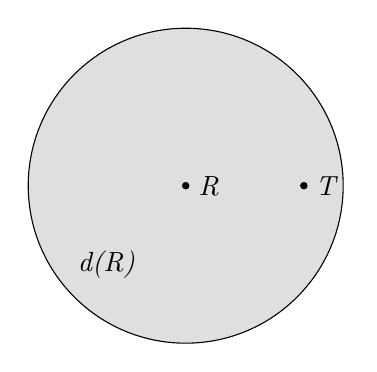
\begin{tikzpicture}
    \draw[fill=lightgray!50!white]   (0,0) circle (2cm);
    \node[] at (-1,-1) {\textit{d(R)}};
    \draw[fill=black]   (0,0) circle (.4mm);
    \node[] at (0.3,0) {\textit{R}};
    \draw[fill=black]   (1.5,0) circle (.4mm);
    \node[] at (1.8,0) {\textit{T}};
\end{tikzpicture}
   \caption{d(R) includes T}\label{fig:tsedryk:1}
 \end{subfigure}
 \hspace{1cm}
 \begin{subfigure}{5cm}
 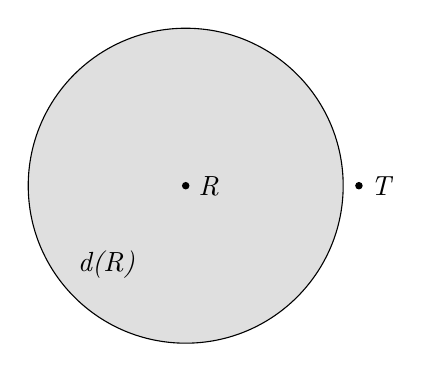
\begin{tikzpicture}
    \draw[fill=lightgray!50!white]   (0,0) circle (2cm);
    \node[] at (-1,-1) {\textit{d(R)}};
    \draw[fill=black]   (0,0) circle (.4mm);
    \node[] at (0.3,0) {\textit{R}};
    \draw[fill=black]   (2.2,0) circle (.4mm);
    \node[] at (2.5,0) {\textit{T}};
\end{tikzpicture}
\caption{d(R) excludes T}\label{fig:tsedryk:2}
 \end{subfigure}
 \begin{subfigure}{5cm}
 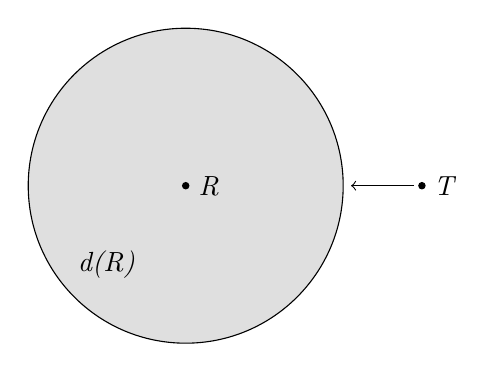
\begin{tikzpicture}
    \draw[fill=lightgray!50!white]   (0,0) circle (2cm);
    \node[] at (-1,-1) {\textit{d(R)}};
    \draw[fill=black]   (0,0) circle (.4mm);
    \node[] at (0.3,0) {\textit{R}};
    \draw[fill=black]   (3.0,0) circle (.4mm);
    \node[] at (3.3,0) {\textit{T}};
    \path[draw,->] (2.9,0) -- (2.1,0);
\end{tikzpicture}
 \caption{T is directed towards d(R)}\label{fig:tsedryk:3}
 \end{subfigure}
 \hspace{1cm}
 \begin{subfigure}{5cm}
 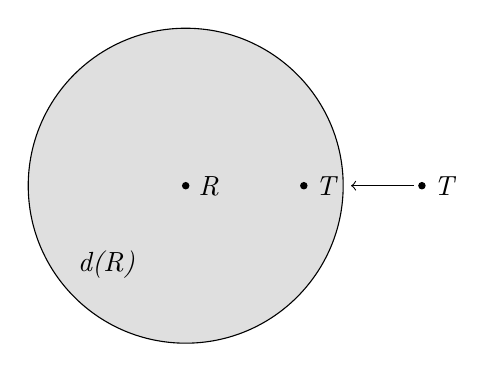
\begin{tikzpicture}
    \draw[fill=lightgray!50!white]   (0,0) circle (2cm);
    \node[] at (-1,-1) {\textit{d(R)}};
    \draw[fill=black]   (0,0) circle (.4mm);
    \node[] at (0.3,0) {\textit{R}};
    \draw[fill=black]   (1.5,0) circle (.4mm);
    \node[] at (1.8,0) {\textit{T}};
    \draw[fill=black]   (3.0,0) circle (.4mm);
    \node[] at (3.3,0) {\textit{T}};
    \path[draw,->] (2.9,0) -- (2.1,0);
\end{tikzpicture}
 \caption{d(R) includes T in an inertia world}\label{fig:tsedryk:4}
 \end{subfigure}
 \caption{Spatial relationships between the domain/sphere of a reference point, \textit{d}(\textit{R}), and a target point (\textit{T})}
\end{figure}


As we can see in \figref{fig:tsedryk:1} and \figref{fig:tsedryk:2}, there are two self-excluding logical possibilities: either \textit{d}(\textit{R}) includes \textit{T} or \textit{d}(\textit{R}) excludes \textit{T}. However, exclusion does not rule out a possibility of including \textit{T} within \textit{d}(\textit{R}) if we add a vector, as in \figref{fig:tsedryk:3}. Assuming inertia, if \textit{T} continuously moves towards \textit{d}(\textit{R}), we can infer from the vector in \figref{fig:tsedryk:3} that \textit{T} will cross the inclusion boundary at some point. That is, even though \textit{T} is not included in \textit{d}(\textit{R}) in the actual world, inclusion is still possible in an “inertia world” \citep[148]{Dowty1979}.\footnote{\citet{Dowty1979} uses an inertia function in his definition of the progressive operator, assuming a branching time model. My use of the term, applied to a conceptual metaphor, is rather informal a this point. Interestingly, the dative does correlate with the imperfective operator in dative infinitive constructions (\sectref{sec:tsedryk:4}), but a detailed account of this correlation in the aspectual domain is beyond the scope of this paper. }  It is thus plausible to differentiate between inclusion in the actual world and the one in an inertia (possible) world, as in \figref{fig:tsedryk:4}. Crucially, motion and the end-point are inferred from the directional vector, but they are not part of the dative meaning itself (see \citetv{chapters/fabregas}).

Possession (as a meta category) can thus be conceptualized as a feature-geo\-met\-ric system in \REF{ex:tsedryk:28}, where the sisters are mutually excluding privative features and dominance corresponds to implication. The terminal nodes are the lexical roots (and their grammatical case features) assumed in \sectref{sec:tsedryk:2.3}.\footnote{My analysis does not contradict \parencitetv{chapters/franco}, who observe that dative morphology can mark inclusion in world languages. It is expected that languages vary at the morphological level (the dative being more or less polysemous). My point is that the dative is not reducible to inclusion universally. Russian makes a clear morphological distinction between locational and directional meanings. For example, Russian cannot mark actual possession using the dative like French (e.g., \textit{ce livre est à moi} ‘this book is mine’; cf. \REF{ex:tsedryk:13}).}


\ea%28
    \label{ex:tsedryk:28}
\begin{forest}
[Possession
    [Inclusion (within) [$\sqrt{\text{at}}$ (genitive)]]
    [Exclusion [Direction (towards) [$\sqrt{\text{to}}$ (dative)]]]
]
\end{forest}
    \z

Finally, in order to bridge the above features with the modal uses of the dative, let me touch upon the notion of control, mentioned in \sectref{sec:tsedryk:1} (see the excerpt from \citeauthor{BjorkmanCowper2016} above \REF{ex:tsedryk:3}). I shall start with a slight detour and provide further details on \textit{d}(\textit{R}) and its content. What class of potential targets can we have? As a conceptual region (in Langacker’s terms), \textit{d}(\textit{R}) includes first of all \textit{R}’s physical body and, depending on \textit{R}’s animacy and human attributes, \textit{d}(\textit{R}) can also include \textit{R}’s living space, personal belongings, social relations and, ultimately, controlled situations. The list of things that can be included in \textit{d}(\textit{R}) seems to be heterogeneous, but all these elements (we may call them “particulars”) can be sorted into two main types, individuals and situations. In situation semantics (\citealt{Kratzer1989}, \citeyear{Kratzer2002}, \citeyear{Kratzer2019}), \textit{d}(\textit{R}) can be thought of as a “thick particular”, as opposed to a “thin particular”. In Kratzer’s own words:

\begin{quote}
We may consider particulars with all their ‘properties’. This gives us the notion of a ‘thick’ particular. Alternatively, we may have a conception of a ‘thin’ particular. A thin particular is a particular with all its ‘properties’ stripped off (the ‘residue’ in more traditional terminology). When we say that a state of affairs is a particular’s having a ‘property’ or two or more particulars standing in some ‘relation’, the notion of a thin particular is involved. Thick particulars are themselves states of affairs (but not every state of affairs is a thick particular, of course). \hfill \citep[613]{Kratzer1989}
\end{quote}

As a thick particular, \textit{d}(\textit{R}) is a set of thin particulars (cf. “entities” in Langacker’s definition). Thin particulars, in their turn, are conceptualized as either individuals (\textit{e}) or situations (\textit{s}). That is, \textit{T} can be of type \textit{s} as well as of type \textit{e}. This distinction will be relevant for us in \sectref{sec:tsedryk:4}, where I will use the same functions and compositional rules as in \sectref{sec:tsedryk:2.3}, but incorporating situations. Exclusion of a situation from \textit{d}(\textit{R}) implies a lack of control over that situation in the actual world. However, adding a vector, as in \figref{fig:tsedryk:3}, we infer that a situation is under control in an inertia world. This is what makes the dative – terminal node  $\sqrt{\text{to}}$  in \REF{ex:tsedryk:28} – a good fit for a modal use. This last point finally brings us to my analysis of possessive modality in Russian.

\section{Possessive modality in Russian}\label{sec:tsedryk:4}

As I have already mentioned in footnote 3, not all dative infinitive constructions in Russian have possessive modality, which is restricted to declarative imperfective clauses, as in \REF{ex:tsedryk:29a}. In \REF{ex:tsedryk:29b}, I show that the verb cannot be perfective. The perfective aspect becomes possible if we add negation, as in \REF{ex:tsedryk:30a}, or use a \textit{wh-}phrase, as in \REF{ex:tsedryk:30b}, but the modal flavour is not the same (see \citealt{Fortuin2007, Tsedryk2018}).

\ea%29
    \label{ex:tsedryk:29}
    \ea\label{ex:tsedryk:29a}
    \gll    {Vane}          {zavtra}       {rano}   {vsta-va-t’}.\\
            Vanja.\textsc{dat}  tomorrow  early  get.up-\textsc{ipfv-inf}\\
    \glt    ‘Vanja has to get up early tomorrow.’
    \ex\label{ex:tsedryk:29b}
    \gll    *{Vane}          {zavtra}       {rano}   {vsta-t’}.\\
            \hspaceThis{*}Vanja.\textsc{dat}  tomorrow  early  get.up.\textsc{prf-inf}\\
    \glt    [the same as in \REF{ex:tsedryk:29a}]
    \z
\z

\ea%30
    \label{ex:tsedryk:30}
    \ea\label{ex:tsedryk:30a}
    \gll    {Vane}         {zavtra}       {rano}   {ne}     {vsta-t’}.\\
            Vanja.\textsc{dat}  tomorrow  early  \textsc{neg}    get.up.\textsc{prf-inf}\\
    \glt    ‘Vanja will not be able to get up early tomorrow.’
    \ex\label{ex:tsedryk:30b}
    \gll    {Vo}    {skol’ko}       {Vane}           {zavtra}         {vsta-t’}?\\
            at    what.time    Vanja.\textsc{dat}  tomorrow    get.up.\textsc{prf-inf}\\
    \glt    ‘At what time should Vanja get up tomorrow?’
    \z
\z

In what follows, I will focus on possessive modality and will not attempt an analysis of the modal flavours in \REF{ex:tsedryk:30}, as this endeavour would take me too far afield. However, the syntactic derivation that I propose below can be applied to all dative infinitive constructions.

In a nutshell, my main idea is that \textit{i}* can create a dative applicative structure on the top of a TP, just like it creates such a structure on the top of an NP; compare \REF{ex:tsedryk:31} with \REF{ex:tsedryk:18}.\footnote{A high applicative structure on the top of a TP is not new. It has already been proposed by \citet{Rivero2009} and \citet{RiveroArregui2012} for involuntary state constructions in Slavic.}

\ea%31
    \label{ex:tsedryk:31}
\begin{forest}
[T*P
    [DP\textsubscript{[DAT]}\\\textit{Vane}]
    [T*P\textsubscript{[s:D][DAT]}
        [T*\textsubscript{[s:D][DAT]}
            [$\sqrt{\text{to}}$\textsubscript{[DAT]}]
            [\textit{i}*\\T\textsubscript{[s:D]}]
        ]
        [TP\\{\textlangle}DP\textsubscript{[case:\_\_]}{\textrangle} \textit{zavtra} \textit{rano} \textit{vstavat’}\\(‘get up early tomorrow’)]
    ]
]
\end{forest}
    \z

Apart from the categorial difference, \REF{ex:tsedryk:31} is different from \REF{ex:tsedryk:18} by its derivational history: it is a raising structure (DP has a copy within TP). This peculiarity of \REF{ex:tsedryk:31} is derived from \citegen{Chomsky2013} labeling algorithm, which resolves labeling ambiguity in cases like \REF{ex:tsedryk:32a}: two maximal projections are merged and do not share any features. In order to label α, we have to merge an extra head H (which projects an HP) and move either XP or YP. Suppose it is XP that has to move, as in \REF{ex:tsedryk:32b}. This movement creates a “discontinuous element” \citep[44]{Chomsky2013}, whose lower copy becomes irrelevant for labeling, and α is labeled as YP.

\ea%32
    \label{ex:tsedryk:32}
    \ea\label{ex:tsedryk:32a}{}
    [\textsubscript{α} XP YP]
    \ex\label{ex:tsedryk:32b}{}
    [\textsubscript{β} XP [\textsubscript{HP} H [\textsubscript{YP} {\textlangle}XP{\textrangle} YP]]]
    \z
\z

We have the same situation in \REF{ex:tsedryk:33a}, where the subject raises from its thematic position (Spec,{\liv}P) and merges with a TP. Since we have an infinitival TP (without agreement features), there are two consequences: (i) DP cannot be case-marked and (ii) α cannot be labeled. We have to merge a case-assigning head. This is where \textit{i}* comes into play. However, it cannot be a bare \textit{i}* (which does not have its own case feature to assign); it has to be \textit{i}* with a case assigning root.

\ea%33
    \label{ex:tsedryk:33}
    \ea\label{ex:tsedryk:33a}{}
    [\textsubscript{α} DP TP]
    \ex\label{ex:tsedryk:33b}{}
    [\textsubscript{β} \textit{i}*\textsubscript{[DAT]} [\textsubscript{α} DP TP]]
    \ex\label{ex:tsedryk:33c}{}
    [\textsubscript{T*P} DP\textsubscript{[DAT]} [\textsubscript{T*P} T*\textsubscript{[DAT]} [\textsubscript{TP} {\textlangle}DP{\textrangle} TP]]]
    \z
\z

For simplicity’s sake, I identify it as \textit{i}*\textsubscript{[DAT]} in \REF{ex:tsedryk:33b}. Note that \textit{i}*\textsubscript{[DAT]} does not have a categorial value at this point, since α is not yet labeled in \REF{ex:tsedryk:33b}. When DP moves (for case reasons), α is labeled as TP, \textit{i}* receives its categorial value (T*), β becomes T*P, DP receives the dative case (checking [s:D]), and we obtain the structure in \REF{ex:tsedryk:33c}. The tree in \REF{ex:tsedryk:31} is the final state of this derivation.

Interpretation of the nodes in \REF{ex:tsedryk:31} is provided in \REF{ex:tsedryk:34}. The main difference between \REF{ex:tsedryk:31} and \REF{ex:tsedryk:18} is that the category expanded by \textit{i}* in \REF{ex:tsedryk:31} is a proposition (\textit{p}). As defined in \REF{ex:tsedryk:34d}, it is a function of type {\textlangle}\textit{s}, \textit{t}{\textrangle}, compared to the NP of type {\textlangle}\textit{e}, \textit{t}{\textrangle} in \REF{ex:tsedryk:23}. Correspondingly, T* in \REF{ex:tsedryk:31} is of type {\textlangle}\textit{e}, {\textlangle}\textit{s}, \textit{t}${\rangle}{\rangle}$ (see \REF{ex:tsedryk:34c}), compared to type {\textlangle}\textit{e}, {\textlangle}\textit{e}, \textit{t}${\rangle}{\rangle}$ of N* in \REF{ex:tsedryk:18} (see \REF{ex:tsedryk:21b}). Just like with the NP, the semantic composition in \REF{ex:tsedryk:34} proceeds by Functional Application in all cases except \REF{ex:tsedryk:34e}, which is derived by Predicate Conjunction. We end up with a T*P, as in \REF{ex:tsedryk:34f}, which has the same semantic type as the TP in \REF{ex:tsedryk:34d}, but with a directional semantics of the dative.

\newpage
\ea%34
    \label{ex:tsedryk:34}
    \ea\label{ex:tsedryk:34a}
    $\left\llbracket \text{i*}\right\rrbracket  = {\lambda}x {\in}$ D\textit{\textsubscript{e}} . \textit{d}(x)
    \ex\label{ex:tsedryk:34b}
    $\left\llbracket \sqrt{\text{to}}\right\rrbracket  = {\lambda}f {\in}$ D\textsubscript{{\textlangle}}\textit{\textsubscript{s}}\textsubscript{,} \textit{\textsubscript{t}}\textsubscript{{\textrangle}} . [${\lambda}y {\in}$ D\textit{\textsubscript{e}} . [${\lambda}x {\in}$ D\textit{\textsubscript{s}} . towards'(f(y))(x)]]
    \ex\label{ex:tsedryk:34c}
    $\left\llbracket \text{T* in \REF{ex:tsedryk:31}}\right\rrbracket  = {\lambda}y {\in}$ D\textit{\textsubscript{e}} . [${\lambda}x {\in}$ D\textit{\textsubscript{s}} . towards'(\textit{d}(y))(x)]
    \ex\label{ex:tsedryk:34d}
    $\left\llbracket \text{TP in \REF{ex:tsedryk:31}}\right\rrbracket  = {\lambda}x {\in}$ D\textit{\textsubscript{s}} . \textit{p}(x)
    \ex\label{ex:tsedryk:34e}
    $\left\llbracket \text{lower T*P in \REF{ex:tsedryk:31}}\right\rrbracket  = {\lambda}y {\in}$ D\textit{\textsubscript{e}} . [${\lambda}x {\in}$ D\textit{\textsubscript{s}} . towards'(\textit{d}(y))(x) ${\wedge}$ \textit{p}(x)]
    \ex\label{ex:tsedryk:34f}
    $\left\llbracket \text{upper T*P in \REF{ex:tsedryk:31}}\right\rrbracket  = {\lambda}x {\in}$ D\textit{\textsubscript{s}} . towards'(\textit{d}(vanja'))(x) ${\wedge}$ \textit{p}(x)
    \z
\z


According to \REF{ex:tsedryk:34f}, situations (in which \textit{p} is true) are directed towards Vanja’s domain/sphere, but Vanja is not their controller, planner, or “director” (in the sense of \citealt[272]{Copley2008}). There is a potentially infinite number of possible situations that could be excluded from Vanja’s domain/sphere. Thus, the remaining step in the computation is to provide the modal base that would restrict all possible situations to those that are relevant in a given context (\textit{c}).\footnote{I abstract away from the accessibility relation here. An articulated account is yet to be developed.}  The modal base (MB), as defined in \REF{ex:tsedryk:35a}, consists of all (contextually salient) preparatory situations (\textit{Prep}) applied to a function of type {\textlangle}\textit{s}, \textit{t}{\textrangle} (cf. “preparatory process” in \citealt[328--331]{CipriaRoberts2000}, following \citealt{MoensSteedman1988}).\footnote{Sentences like \REF{ex:tsedryk:29a} imply a topic situation, as in (i) (in brackets). Preparation for the main event (Vanja’s early rising tomorrow) is an alternative to the topic situation (Vanja’s sitting for long time).

\ea%i
    \gll    {Vane} {zavtra} {rano}   {vsta-va-t’}  (on {ne} {možet} {s} {vami}  {dolgo}       sidet’).\\
            Vanja.\textsc{dat}  tomorrow  early get.up-\textsc{ipfv-inf} he \textsc{neg}    can    with you   long.time  to.sit\\
    \glt    ‘Vanja has to get up early tomorrow (he can’t sit with you for long time).’
\z
}~Functional Application between \REF{ex:tsedryk:35a} and \REF{ex:tsedryk:34f} results in \REF{ex:tsedryk:35b}, which is read as follows: for all x, such as x is a preparatory situation, it is true that x is directed towards Vanja’s domain/sphere, and \textit{p} holds. The tree in \REF{ex:tsedryk:36} shows this last step of the derivation in syntax (a merger between C, which provides the modal base, and T*P).

\ea%35
    \label{ex:tsedryk:35}
    \ea\label{ex:tsedryk:35a}
    $\left\llbracket \text{MB}\text{Prep}\right\rrbracket$\textit{\textsuperscript{c}} = ${\lambda}f {\in}$ D\textsubscript{{\textlangle}}\textit{\textsubscript{s}}\textsubscript{,} \textit{\textsubscript{t}}\textsubscript{{\textrangle}} . ${\forall}x {\in}$ D\textit{\textsubscript{s}}, \textit{Prep}(x) ${\rightarrow}$ f(x)
    \ex\label{ex:tsedryk:35b}
    $\left\llbracket \text{MB}\text{Prep}\right\rrbracket$\textit{\textsuperscript{c}} ($\left\llbracket\text{upper T*P in \REF{ex:tsedryk:31}}\right\rrbracket $) = ${\forall}x {\in}$ D\textit{\textsubscript{s}}, \textit{Prep}(x) ${\rightarrow}$ [towards'(\textit{d}(vanja'))(x) ${\wedge}$ \textit{p}(x)]
    \z
\z

\ea%36
    \label{ex:tsedryk:36}
\begin{forest}
[CP\textit{\textsubscript{t}}
    [C\textsubscript{${\langle}{\langle}$}\textit{\textsubscript{s}}\textsubscript{,} \textit{\textsubscript{t}}\textsubscript{{\textrangle},} \textit{\textsubscript{t}}\textsubscript{{\textrangle}}\\MB\textit{\textsubscript{Prep}}]
    [T*P\textsubscript{{\textlangle}}\textit{\textsubscript{s}}\textsubscript{,} \textit{\textsubscript{t}}\textsubscript{{\textrangle}}\\\textit{Vane zavtra rano vstavat’}\\(‘Vanja.\textsc{dat} get up early tomorrow’)]
]
\end{forest}
    \z

The imperfective entails that every preparatory situation is interpreted as an inertia situation (without interruptions), which inevitably reaches Vanja’s domain/sphere in a corresponding inertia world (cf. “preparatory inertia” in \citealt[324]{RiveroArregui2012} and \citealt[327]{ArreguiRiveroSalanova2014}).\footnote{\citet[325]{RiveroArregui2012} claim that the imperfective in Russian (and West Slavic) does not have access to preparatory inertia, as it cannot have intentional readings. This claim is partly true. Indeed, the imperfective in Russian cannot have intentional readings in the past tense, as shown in (i).

\ea%i
    \gll    *Vanja         vsta-va-l           v   pjat’   utra           poka   ne    otmenili       trenirovku.\\
            \hspaceThis{*}Vanja.\textsc{nom}   get.up-\textsc{ipfv-pst}   at  five   of.morning   until     \textsc{neg} canceled.\textsc{3pl}   practice\\
    \glt    \textit{Intended}: ‘Vanja was planning to get up at 5 am until the practice was   canceled.’
    \z

However, Rivero \& Arregui do not consider Russian dative infinitive constructions, as in \REF{ex:tsedryk:29a}, which do have an intentional reading (e.g., the intention is to get up early tomorrow). There is some “clash” between the imperfective and the past tense in Russian, preventing intentional readings in cases like (i), but otherwise the claim that preparatory inertia is not available for the imperfective in Russian is too strong.}

To summarize, possessive modality in Russian is represented by a subset of dative infinitive constructions, declarative and imperfective. My goal in this section was to show that there is a parallel between the datives introduced above NP and those introduced above TP. In the latter case, the dative entails that a situation is not under control in the actual world, but can be brought under control in an inertia world. This possibility is derived from the directional semantics of the dative argument introducer in the context of inertia situations entailed by the imperfective.


\section{Conclusion}\label{sec:tsedryk:5}

Predicative possession and possessive modality show a striking similarity, but they also differ with respect to case marking in \textsc{be}{}-languages. Possessive modality correlates with the dative case. \citet{BjorkmanCowper2016} propose to capture the attested similarity, using a morpho-semantic feature, [\textsc{incl}], which encodes inclusion within an abstract domain/sphere. As for the dative case, they suggest that it is a spell-out of [\textsc{incl}] bundled with a modal feature, [\textsc{root}] or [\textsc{epist}]. I have shown that this analysis, when applied to Russian, has a number of limitations. First, it makes false predictions with respect to locative (actual) possessors. Second, it has little to say about the predicative possession with dative (prospective) possessors. I suggested that the link between predicative possession and possessive modality should be established via directional semantics of the head introducing this dative in two syntactic contexts, NP (sets of individuals) and TP (sets of situations). In my analysis, I used \citegen{WoodMarantz2017} argument introducer and two spatial roots,  $\sqrt{\text{at}}$  and  $\sqrt{\text{to}}$. Possessive modality is derived from the directional semantics of the second root and inertia situations entailed by the imperfective. My analysis leads to a hypothesis that possessive modality in other \textsc{be}{}-languages could also be linked to directional semantics (even if a language does not use the same datives as Russian). The dative case used in possessive modality structures is not a trivial matter of language-specific spell-out rules; it calls for a careful crosslinguistic investigation.



\section*{Abbreviations}
The abbreviations used in the glosses of this chapter follow the Leipzig Glossing Rules.

\section*{Acknowledgements}

I would like to thank two anonymous reviewers for their detailed comments on the earlier draft.

\sloppy\printbibliography[heading=subbibliography,notkeyword=this]
\end{document}
